\documentclass{report}
\usepackage{xcolor}
\usepackage{epigraph}
\usepackage{ulem}
\usepackage{graphicx}
\graphicspath{{images/}}
\usepackage[screen,code,rightpanel,gray,sectionbreak]{pdfscreen}
     \margins{.65in}{.65in}{.65in}{.65in}
     \overlay{overlay2.pdf}
     \paneloverlay{overlay4.pdf}
     \screensize{6.25in}{8in}
%\emblema{PotionWarsTitleScreen}
\urlid{www.spankingrpgs.blogspot.com}

%\titlehead{{\centering\includegraphics{image}}
\title{
\includegraphics{title}}
\author{Andrew Russell}

\date{\today}

\begin{document}
\textit{Pandemonium Cylce: The Potion Wars} is intended for adults only. Spanking and other erotic content depicted in this game and all related material,
including but not limited to manuals, readmes, and images, are fantasies and intended for adults only. Nothing in this game should be interpreted as advocating any
form of non-consensual spanking or the spanking of minors. I firmly believe that non-consensual spankings are abuse in any relationship, including but not
limited to friendships, marriages, and child-rearing.

--Andrew Russell

\chapter*{Prologue}
\label{ch_prologue}
Alis Silver entered the university library. She was a short, mousy girl with very pale, lightly freckled skin. Her straw-colored hair was pulled back
into a ponytail, and she was fairly
short and thin. She wore a plain t-shirt, a pair of jeans, and sneakers. She wore minimal make-up, just enough to obscure the study-induced bags under her eyes. 

She 
smiled hesitantly as she approached the library desk. Mrs. Summers, a tall woman in her mid-fifties, stood behind the desk. She kept her gray hair pulled 
back into a neat grey bun, and a pair of small reading glasses sat on the bridge of her nose. Her eyes swept over her library, which was filled with the quiet murmur of 
students
hard at work, hard at sleeping, and hard at internet surfing. A wooden ruler sat on the desk next to her, as if the signs posted at the library entrance weren't warning
enough of the consequences of misbehavior.

The librarian's stern gaze dissolved into a warm smile when she saw Alis, and Alis' nerves vanished. ``Ah, good afternoon Alis. You're not scheduled to work
today. I don't suppose you're just here to visit little old me?"

Alis smiled. She'd spent the past two years working for Mrs. Summers as part of her work-study. Mrs. Summers clearly liked her, and Alis viewed the older woman as sort of a 
second mother. But that didn't stop Alis from feeling a bit nervous whenever she saw the strict old librarian. She cared too much about earning the woman's respect to feel 
otherwise. Her many memories of Mrs. Summers applying that ruler to rule-breaking students (though not to her, thank the Mother), didn't help either.


``Sorry Mrs. Summers," said Alis. ``Much as I'd like to, I'm much too busy. Taking a history class, and for my term project, I have to write a paper about some of
my ancestors."

Mrs. Summers gave Alis a stern look. ``Waiting until mid-October to start, hmm?"

``No, ma'am," said Alis quickly, her hands twitching, and her eyes flicking to the ruler. ``I spent September researching my geneology, and choosing the ancestors I'd
like to write about."

``Ah," said Mrs. Summers. Her expression did not soften. ``You're not spending all your time studying, are you dear? Last thing you want is to spend the entirety of 
your twenties working."

Alis frowned, and crossed her arms over her chest. ``I try, but it's so hard. I have homework, and tests, and term projects, and the way my professors talk everything is
super important forever\ldots"

Mrs. Summers nodded, her expression turning sympathetic. ``I understand, dear. A few things to remember. Your entire life, people will want you to do things, and they'll
be insisting that it's super important forever. And it may be to them, but that doesn't mean it is to you. Your professors are professors precisely because they think what
they're teaching is extremely important, and they're trying to mold all of you into becoming experts in their chosen subjects. Thing is, just because they think their subject
is worth mastering, doesn't necessarily mean you should. There's a reason we have
A's, B's, C's and so on, instead of just pass-fail. You don't need to get an A in every subject."

Alis smiled cheekily. ``Does that also apply to my work-study?"

``For the other students, yes," said Mrs. Summers. ``But not for you. I find you giving anything less than one hundred percent, and I'll smack your little bottom."

Alis swallowed.

Mrs. Summers' stern look dissolved into a smile. She reached over the desk and patted Alis on the arm. ``I'm just teasing, dear. Yes, that applies to your work-study too. 
You could ease off a little bit, and your work would still be more than adequate."

``I know," said Alis. ``You're just scary, even when you're joking."

Mrs. Summers' eyes sparkled. ``I certainly hope so. There are three people you should always be a little bit scared of: your mother, your boss, and your librarian."

``And you're two of those," said Alis ruefully. ``Yay me."

``Now, which ancestors have you decided to research?" asked Mrs. Summers.

Alis pulled her backpack around, and unzipped it. She rooted around inside it for a moment, and pulled out a crumpled sheet of paper. She held it out to the
librarian. 

Mrs. Summers looked at the crumpled paper, then gave Alis a scolding look. ``Someone needs to work on organizing her backpack. I don't suppose your room is any better?"

Alis smiled sheepishly. ``Messiness is not a crime."

``In my day it was," said Mrs. Summers, as she smoothed out the paper. ``The RA would have weekly inspections. If your room wasn't up to snuff, it was the paddle
for you."

``Yes, yes, and then you had to walk to school with a blistered bottom, through the snow, rain, and tornados, uphill both ways," said Alis rolling her eyes.

``You are a cheeky girl aren't you," said Mrs. Summers. She read the names on the paper. Her eyebrows went up. ``You have a very interesting family."

``I checked and double-checked," said Alis quickly. ``I swear it's right."

``Not doubting you dear. In fact, your last name is exactly that given to Silvestone bastards, back when branding children with their fathers' promiscuity was a thing," 
said Mrs. Summers.

Alis deflated a little. ``I'm descended from a bastard?"

``Most of us are dear." Mrs. Summers typed up something on her computer. ``For as long as sexual reproduction has been a thing, men have been bad at keeping it in
their pants. It's like evolution encourages it or something."

``Yes," said Alis, a touch warily, not quite sure how to take Mrs. Summers' comment.

Mrs. Summers pulled out a pencil, grabbed a scrap of paper, and quickly wrote something down. ``Come on, we've got a few very good books about these four."

``I can find them myself-" said Alis.

``While I'm sure you could, your ancestors have been at the center of some very controversial times," said Mrs. Summers, picking up her ruler, and coming around the 
desk. She began leading
Alis deeper into the library. ``For every honest historian trying to understand what actually happened, there are four trying to force history to fit their own twisted
worldviews."

``Why?" asked Alis, hurying to keep up with the librarian's long strides.

``Because we're still dealing with their repurcussions today," said Mrs. Summers.

``But, some of these were centuries ago," said Alis. ``The Potion Wars and Schism happened before Domania even existed."

``Indeed," said Mrs. Summers, smirking at Alis. ``Makes you worried when selfish, short-sighted men use their supposed rights as an excuse to trample on the rest of 
us. Is it just a temporary setback, or will the next five, six, seven generations be trampled too?" 

Alis nodded uncomfortably. 

``Guess I am flirting a bit with talking politics aren't I?" said Mrs. Summers. ``Sorry."

The two stepped up onto the third floor, and entered the history section. There were two girls at a nearby table, their backs to Mrs. Summers and Alis. 
One was sitting, and the other bent over the sitting girl's shoulder, a bright purple thong sticking out the top of her low-rise jeans. They
each had a headphone in one ear, and they were watching something on the computer.

Mrs. Summers' lips thinned. She approached the bent over girl, and slapped the girl's bottom with her ruler.

The girl yelped and jumped up, her hands snapping back to clutch at her bottom. The earbud popped out of her ear. She spun around, her wide brown eyes widening further.

``Mrs. Summers," said the girl quickly. ``I-"

``I believe I sent you up here to shelve books, Miss Murphy," said Mrs. Summers. Her eyes lit suggestively on a nearby, still very full bookcart. ``Not watch videos with
your friend."

``I'm sorry, it was just the one-" said the girl quickly, rubbing her stinging bottom.

``Must be a very long video then, since I sent you up here ten minutes ago, and the cart is hardly touched," said Mrs. Summers, tapping her ruler lightly against her own
thigh. ``By the way, that cart has computer science books on it. Last I checked, computer science is on the fourth floor."

Pauline Murphy exchanged an anxious look with her friend, then glanced at Alis, who was nervously twisting her shirt as she watched the scene unfold. Pauline began chewing 
her lower lip, as she looked at Mrs. Summers, who seemed to have grown ten feet.

``We will talk about your work ethic when I'm done helping Alis," said Mrs. Summers. 

Pauline's friend winced, while Pauline went pale. ``I swear, it won't happen again. Please Mrs. Summers-"

``I've noticed in the past that it takes you an unusually long time to put away books."

``But I'm-"

``Even when allowing for the fact that you're still new. How many
times have you let one of your friends distract you with videos of-" Mrs. Summers peered at the laptop. ``Music videos of dancing shirtless men with an impressive
musculature?"

``Once or twice," mumbled Pauline, scuffing her foot against the carpet, her cheeks bright red.

``I see," said Mrs. Summers. Her voice softened somewhat. ``Well, get those books shelved. And don't worry too much about your punishment. It'll sting, and you'll be sitting 
gingerly for the next few hours, but you should be fine by tomorrow."

Pauline looked at Mrs. Summers with wide eyes, anxiously biting her knuckle.

``And pull up your pants, before I pull them down," said Mrs. Summers brusquely, walking past the two girls, Alis hurrying to keep up with her.

Alis glanced over her shoulder, and could see Pauline hiking up her jeans, while her friend tittered. Pauline smacked the other girl on the shoulder.

Meanwhile, Mrs. Summers walked through the library stacks with a strange expression. It wasn't worship, not quite. Rather, it was the kind of serenit associated with places of
great sacredness and peace. She reverently ran her fingertips along the book spines. ``I love walking through the library
stacks. So much knowledge. So much scholarship. Do you know how long six thousand years is, Alis?"

``Um, a long time?" asked Alis.

``You have no idea," said Mrs. Summers. She stopped, and began pulling books from the stacks. ``Six thousand years. Of people, just like you or I. Going through their days.
Loving, laughing, yelling, fighting, eating, drinking. Playing games, having sex, raising children. Getting married, having their hearts broken. Being betrayed, 
abandoned, supported, and protected. And yet, at the same time it's an eyeblink! There were hundreds of thousands of years of human history before we developed writing. 
And before
that, billions of years. Of life of all shapes and sizes living and dying. Of molten rock, and stardust. The human mind can't comprehend it. Neither can the elven, for all
their posturing."

Mrs. Summers carried the four books to a nearby table, and set them down. She spread them out for Alis to see the titles.

\textit{Pandemonium Cycle: The Potion Wars.} 

\textit{Pandemonium Cycle: Matirian Schism.} 

\textit{Pandemonium Cycle: Tears of Blood.} 

\textit{Pandemonium Cycle: The Bloodwar.}

``Pandemonium Cycle?" said Alis. ``But I thought these were supposed to be works of history."

``\textit{Pandemonium Cycle} isn't just the name for Matirian mythology," said Mrs. Summers.  ``It's also the name for a rather outdated historical model. The model argued 
that there were long periods of stability that would
then rapidly degenerate into pandemonium, out of which would emerge the foundations for a new period of stability. Modern historians generally reject the model as too
simplistic. However, these books do still provide solid history. Some of the information is of course a 
bit outdated, but they'll still provide a great foundation before you start digging through all the cruft."

Alis nodded.

``By the way, you're in charge of the history section, yes?" asked Mrs. Summers.

``Yes," said Alis, her heart-skipping a beat. Did she mess up somehow?

Mrs. Summers' hand clapped against Alis' small bottom. 

``Eep!" cried Alis, her hands flying back to shield her stinging tush.

``I noticed you misfiled a book on the reign of King James the Wiser," said Mrs. Summers. ``That should be with the rest of the books on the history of Silvania, \textit{not} 
Albion."

``I must have gotten my James' confused," said Alis sheepishly.

``Double-checking the call number would have helped you check your mistake," said Mrs. Summers wryly. ``It is, after all why it's there."

``Sorry ma'am," said Alis, clutching her bottom and eyeing the ruler fearfully.

``Relax dear. A misfiled book is hardly a spanking offense," said Mrs. Summers smiling fondly. ``A light smack maybe, but certainly not a spanking. I'll get it filed 
correctly. You focus on your research."

Alis nodded. She rubbed away some of the lingering sting, while the librarian disappeared back into the stacks. She shuddered. A single handsmack
stung bad enough. She couldn't imagine how bad it was going to be for Pauline!

Alis pushed away thoughts of Pauline's impending punishment, and pulled out a chair. She sat down, and pulled out her notebook, and pencils. Then,  she opened the 
first book\ldots

\maketitle
\tableofcontents

\chapter{Introduction}
\label{ch_introduction}
\epigraph{Alright. Ready for some deep sounding advice that's actually
blatantly obvious? Good, 'cause I'll be giving you a lot of that.}{Reyna of Chengue}


The city of Avaricum is 
a mess; everything exists in shades of gray, and the ``right thing," whatever that means, is rarely obvious. The men and women on both sides fight with noble, 
selfish, short-sighted, 
wise and above all \emph{human} 
motivations. You'll find yourself caught in a floodtide of love and hate, forgiveness and vengeance, honesty and corruption. Within this morass, it will be up to you to 
determine which injustices can be endured, and which must be fought. 

Once you've made your choice you will find yourself thrown into war between friends turned
enemies, and enemies turned friends. Who knows, perhaps you'll be able to change the course of history and help usher in a new era of peace and prosperity. Or maybe blood 
will flow freely down the streets because of your misguided actions. Or maybe you'll have no impact at all. Perhaps history
will march onwards to a seemingly inevitable conclusion with little regard for the hopes and dreams of one poor adventurer.

Oh, and you'll get spanked. A lot. You'll also spank people. A lot.

So draw your sword, light your fist on fire, and make sure you've got your paddle. The city of Avaricum awaits!

\chapter{The Game Window}
\label{ch_game_window}
\epigraph{Never trust your eyes alone. You have six senses: Five mundane, and one magical. Use them!}{Reyna of Chengue}

The \textit{Pandemonium Cycle: The Potion Wars} viewscreen is split into two pieces:
\begin{itemize}
    \item \verb|World View| - where you'll see everything that your character sees, hear everything your character hears, and feel everything your character feels
    (may the Mother have mercy upon your bottom).
    \item \verb|Command View| - provides a list of valid commands. The commands you can give depend on where you are: in town, talking to someone,
    at a shop, in battle, in a dungeon, etc. Within each command will be a character wrapped in parenthesis (usually the first character). This is the character you press
    to execute the command. There are some special character sequences that represent particular keys:
        \begin{itemize}
            \item \verb|Esc| - represents the Escape key.
            \item {\color{green!50!black}\texttt{<==}} - represents backspace. Note that this is not usually wrapped in parenthesis, because it cannot be mistaken for part of 
            a name.
            \item \verb|Enter| - represents the enter key.
            \item \verb|#| - Used to indicate you should select a number (if a multi-digit number is required, you will be allowed to enter multiple digits).
        \end{itemize}
\end{itemize}

\section{Townmode}
\label{sec_townmode}
    In town mode, the player is moving about town, and interacting with people. The player will never have to worry about combat in town mode. Figure~\ref{fig_townmode}
    shows what the town mode screen looks like.

    \begin{figure}[h!]
        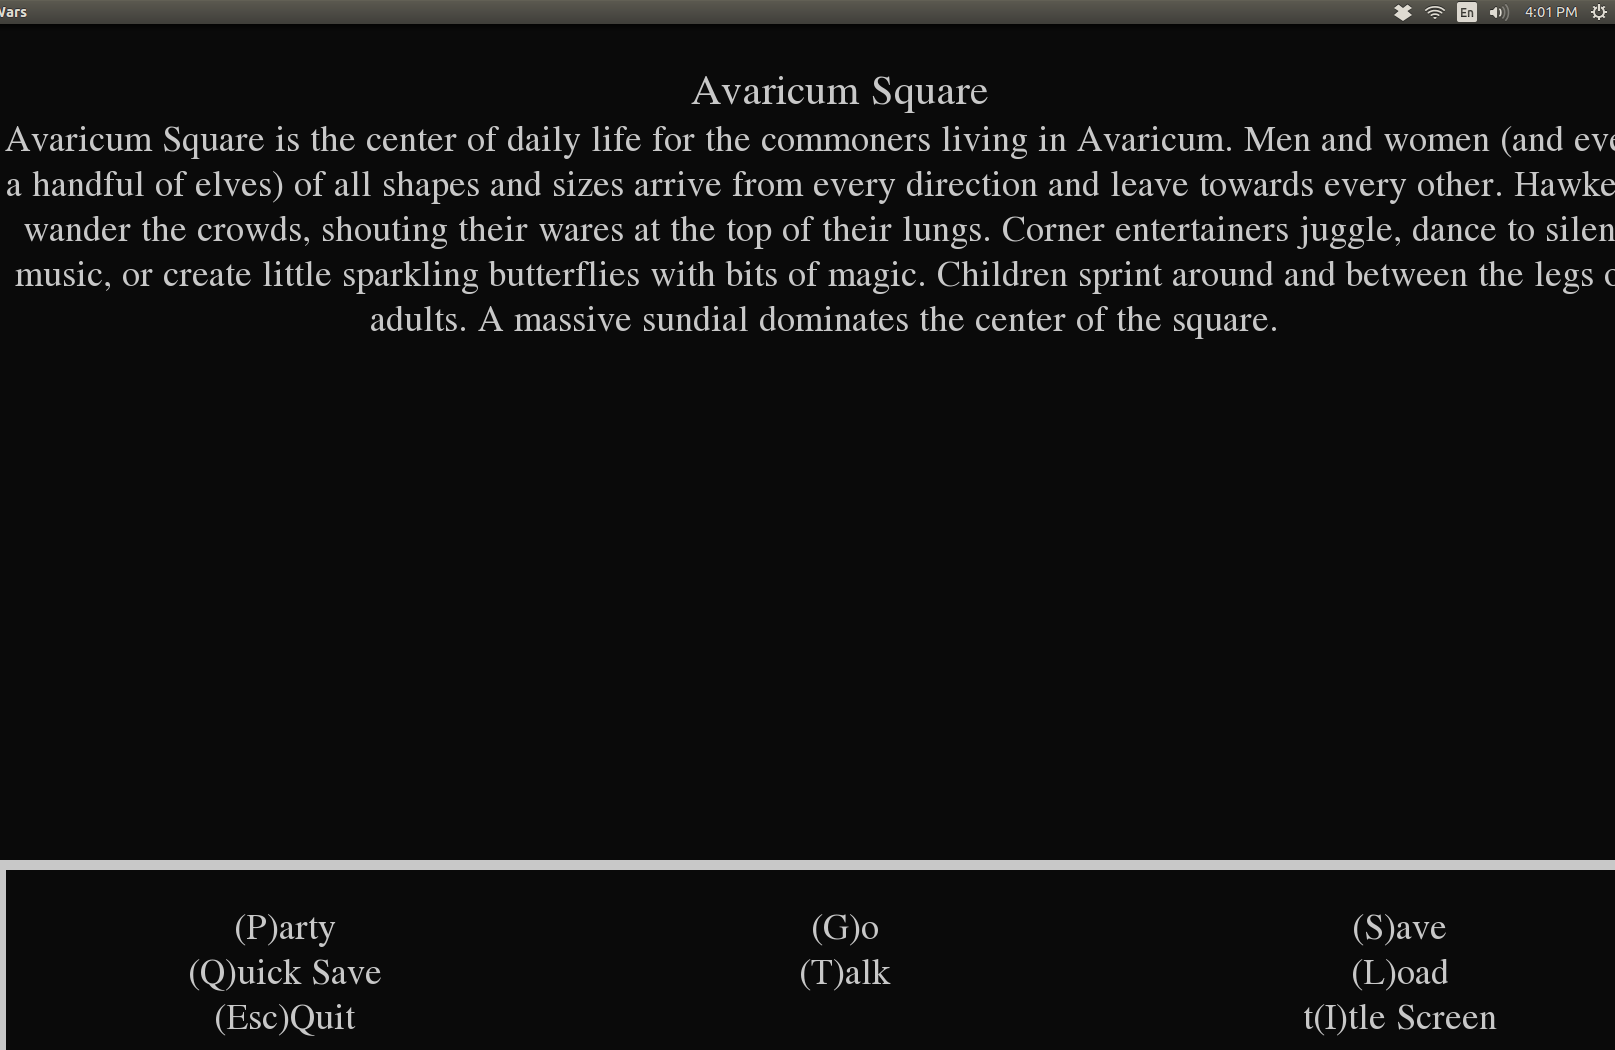
\includegraphics[width=\textwidth]{townmode}
        \caption{I hope the sundial set up a safeword beforehand.}
        \label{fig_townmode}
    \end{figure}

    \begin{itemize}
        \item \verb|(P)arty| - Selected by pressing \verb|P|, the party command allows 
            the player to view the characters currently in their party.
        \item \verb|(G)o| - Selected by pressing \verb|G|, allows the player to go to
        a different location.
        \item \verb|(S)ave| - Allows you to save your game.
        \item \verb|(Q)uick Save| - Saves your game to a file called \verb|quick|.
        \item \verb|(T)alk| - Allows you to talk to someone. If there is no one to
            speak to, this command does nothing.
        \item \verb|(L)oad| - Allows you to load a saved game.
        \item \verb|(Esc)Quit| - Pressing the \verb|Escape| (\verb|Esc| on many 
        keyboards), allows you to close the game (you will be asked if you want to 
        save first).
        \item \verb|t(I)tle Screen| - Note here that the \verb|I| is wrapped in 
        parenthesis, \emph{not} the \verb|t|. By pressing \verb|I| you may return to
        the title screen (you will be asked if you'd like to save first).
        \item \verb|(M)odify Quick Spells|  - Allows you to change which spells are stored as quick spells. The player can have up to 12 quick spells (one for each function key). Your quick spells 
            default to:
            \begin{itemize}
                \item \verb|F1| - Firebolt
                \item \verb|F2| - Weaken
                \item \verb|F3| - Heal
                \item \verb|F4| - Spectral Spanking
            \end{itemize}
    \end{itemize}
    Each time you learn a new spell, that spell will be added to the next available quick spell, so long as you have quick slots available.

\section{Conversation}
\label{sec_conversation}

    Conversation works in the form of a give and take. NPC's will say or do something, then the player will have a chance to respond. The player selects the appropriate
    response by selecting a number. Much of the time, event text will be split across multiple pages, in which case the player presses enter to move through the text 
    until reaching a choice. Note the \verb|(#)| to select a conversation choice. Furthermore, the PC may say things without the player explicitly selecting them.
    Typically, these responses will be either fairly innocuous ("I'm doing alright, how are you?") or will be a reasonable response based on the previous choice made by the
    player (i.e. if you selected a rather bratty response, the PC may act bratty on her own). 

   \begin{figure}[h!]
        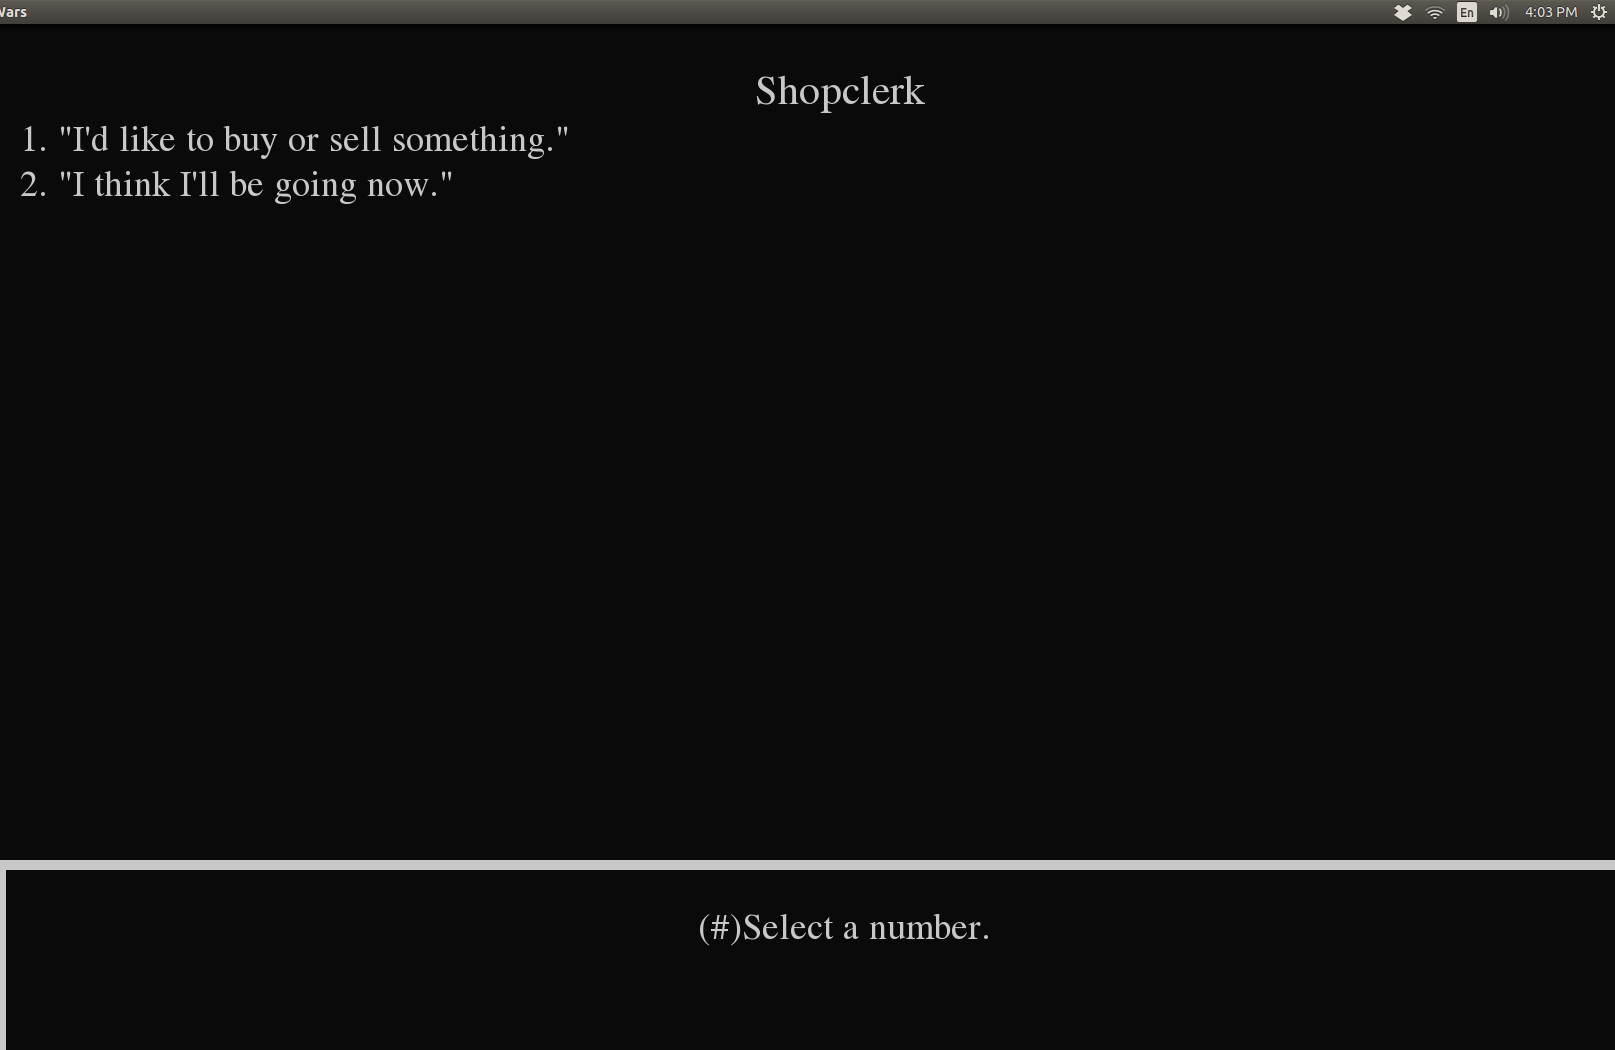
\includegraphics[width=\textwidth]{talking}
        \caption{Even broke adventurers like to go shopping.}
        \label{fig_shopping}
    \end{figure}
    
    Best think carefully about what you say.
    Many of the people you meet have long memories, and while most conversations are inconsequential in the long run, some may have lasting impacts on your bum (also 
    on your path through the game)!

\chapter{Character Screen}
\label{ch_chararacter_screen}
\epigraph{If you want to last
more than five seconds, you better know how to maximize your strengths, and 
minimize your weaknesses. Because you better believe your enemies will be 
minimizing your strengths, and maximizing your weaknesses}{Reyna of Chengue}

\subsection{Gameplay vs. Story}
Magic permeates this world much like oxygen permeates our own. As a result, every living thing on the planet has adapted to use magic to enhance their physical capabilities. As a result, even the 
average person is capable of olympic level feats. Highly experienced warriors can go toe-to-toe with Spider-Man. Even at relatively low levels, magic becomes a much more important factor
than mundane strength (so a five foot tall, 100 pound girl can hold her own in a wrestling match with a six foot tall, 350 pound man). Furthermore, every person has a store of magic called health that 
gives them a healing factor, similar to Wolverine's, except once a person runs out of health, they are no longer capable of healing themselves.

However, using magic to push your body to superhuman levels is \emph{very hard} on your body. As a result, people's bodies have adapted so that they only draw on that power in extreme situations 
(i.e. combat). In their average, day-to-day lives, these people are no stronger, faster, or more resilient than you or I (though many of them are probably in better shape). 

This can lead to rather bizarre situations, like a five foot, 100 pound girl flinging a 6 foot, 350 pound gorilla of a man through a wall, and then fifteen minutes later getting hauled over her 
boyfriends knee (whose half the weight of the aforementioned gorilla-man) and spanked like a naughty schoolgirl.

\subsection{Stats}
Figure~\ref{fig_char_screen} displays the character screen.

\begin{figure}[h!]
    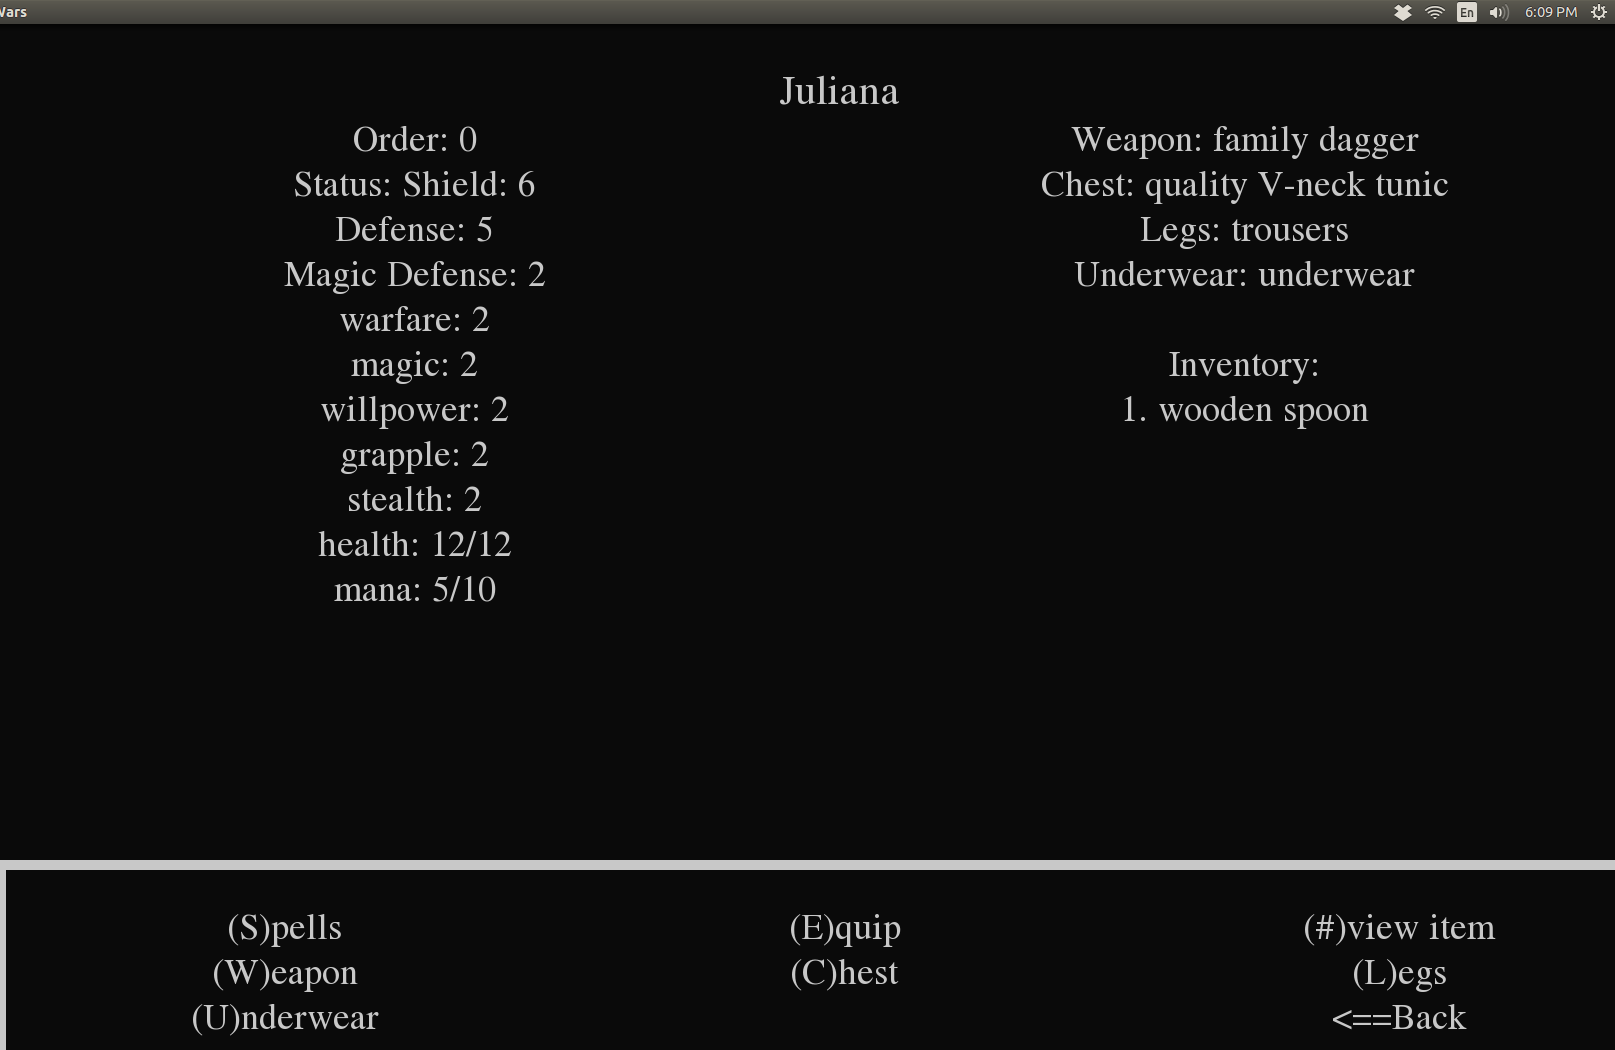
\includegraphics[width=\textwidth]{character_sheet}
    \caption{I look pretty, oh so pretty.}
    \label{fig_char_screen}
\end{figure}

The top of the screen displays the currently displayed character's name. The left 
side contains the following information:

\begin{itemize}
    \item \verb|Order| - An Order is a special ability that some people have. Think
    of it as an adrenaline rush on steroids. When a person with an order faces
    an enemy more powerful than they are (i.e. a dungeon boss), their bodies will unleash an extra large
    burst of adrenaline. This adrenaline will trigger a burst of magical power 
    (called surging). These surges do different things depending on the order of
    the person. 
    The orders are, from common to rare:
    \begin{enumerate}
        \setcounter{enumi}{-1}
        \item Nothing. Person does not surge.
        \item Give all your enemies a small penalty to all stats.
        \item Give you and your allies a small bonus to all stats
        \item Wrap all enemies in a bubble of hostile magic that leaches away health 
        each round.
        \item Wrap all allies in a bubble of soothing magic that restores health
        each round.
        \item Cut all enemies' health and mana in half.
        \item Fully restore all allies' health and mana.
    \end{enumerate}
    \item \verb|Status| - What statuses (good and bad) the character is currently 
    inflicted with. Next to each status is a number. This number is how 
    many turns the status has left. In combat, a single turn is exactly a single
    round of combat. Outside of a combat, a single turn corresponds to a single
    press of an arrow key.
    \item \verb|Defense| - Your character's protection against physical attacks. 
    Influenced by the \verb|Warfare| stat, and your character's equipment.
    \item \verb|Magic Defense| - Your character's protection against magical 
    attacks.
    Influenced by the \verb|Magic| stat, and your character's equipment.
    \item The player has two types of stats: Primary and Secondary. High secondary stats are key to defeating enemies. High primary stats are key to having high secondary stats.
        \begin{itemize}
        \item \verb|Primary|:
            \begin{itemize}
                \item \verb|Strength| - How physically strong your character is. In the heat of combat, a warrior's strength is primarily fueled by magic, not physical muscles. Purely physical
                    processes are only used in relatively low stress, day-to-day activities. Each point gives you two points of \verb|grapple| and one point of \verb|warfare|.
                \item \verb|Dexterity| - How agile your character is. Each point gives you two points of \verb|warfare| and one point of \verb|grapple|.
                \item \verb|Willpower| - How strong your character's mind is. Each point gives two points of \verb|resilience| and one point of \verb|magic|.
                \item \verb|Talent| - How powerful your character's explicit magic is. Each point gives two points of \verb|magic| and one point of \verb|resilience|.
                \item \verb|Alertness| - How aware your character is. Each point gives two points of \verb|stealth|. Half of your Alertness is also added to your character's initiative in combat. 
                    This improves the chances of your character acting early in combat, regardless of the chosen action.
                \item \verb|Health| - A store of magic that your body automatically uses to
                instantly repair any serious physical damage. Note that this is \emph{serious}
                damage, in particular large gashes, serious internal damage, broken bones,
                etc. Bruises and welts are not serious enough to trigger it. Sorry, no 
                magical protection from spankings for you. When a character reaches zero health,
                their body will trigger a final burst of magic to heal all injuries. While this ensures
                the character won't die of any lingering wounds, it also leaves them weak as a kitten, and unable to continue fighting until they've been resparked 
                (``resurrected" in standard RPG parlance).
                \item \verb|Mana| - A store of magic used to cast spells.
            \end{itemize}
        \item \verb|Secondary|:
            \begin{itemize}
                \item \verb|warfare| - How good you are at physical combat. Influences your
                physical damage and defense.
                \item \verb|magic| - How good you are at casting spells. Also measures your
                natural defenses against magic.
                \item \verb|resilience| - Makes your status spells more
                effective, and makes it harder for enemies to inflict you with negative 
                statuses.
                \item \verb|grapple| - How good you are at grappling an opponent (see Chapter
                ~\ref{ch_combat} for details on grappling).
                \item \verb|stealth| - How stealthy you are. A higher stealth increases the 
                chances that you will ambush your enemies, rather than your enemies ambushing
                you. Will also influence the \verb|Hide| command once that has been implemented.
            \end{itemize}
    \end{itemize}
\end{itemize}

    The righthand side is the following information:
\begin{itemize}
    \item \verb|Weapon| - The character's weapon. See Chapter~\ref{ch_combat} for
    more details about the types of weapons.
    \item \verb|Chest| - Armor/clothing that covers the chest and upper body.
    \item \verb|Legs| - Armor/clothing that covers the legs. 
    \item \verb|Underwear| - Your character's underwear. Whether or not a female
    character wears any form of bra is up to the player, it is not explicitly tracked
    by the game.
    \item \verb|Inventory| - Items your character is currently carrying.
\end{itemize}

\chapter{Dungeon}
\label{ch_dungeon}
\epigraph{If you ever find yourself in dangerous territory surrounded by enemies, 
then whatever you do, don't get lost.}{Reyna of Chengue}

    Much of the game will be spent in dungeons (not the sexy kind). The term ``dungeon" is used rather loosely. Dungeons may be as varied as towns, forests,
    caves, and Evul Lairs. However, they all look the same (see Figure~\ref{fig_dungeon}) because I'm a writer/programmer, not an artist!
    \begin{figure}[h!]
        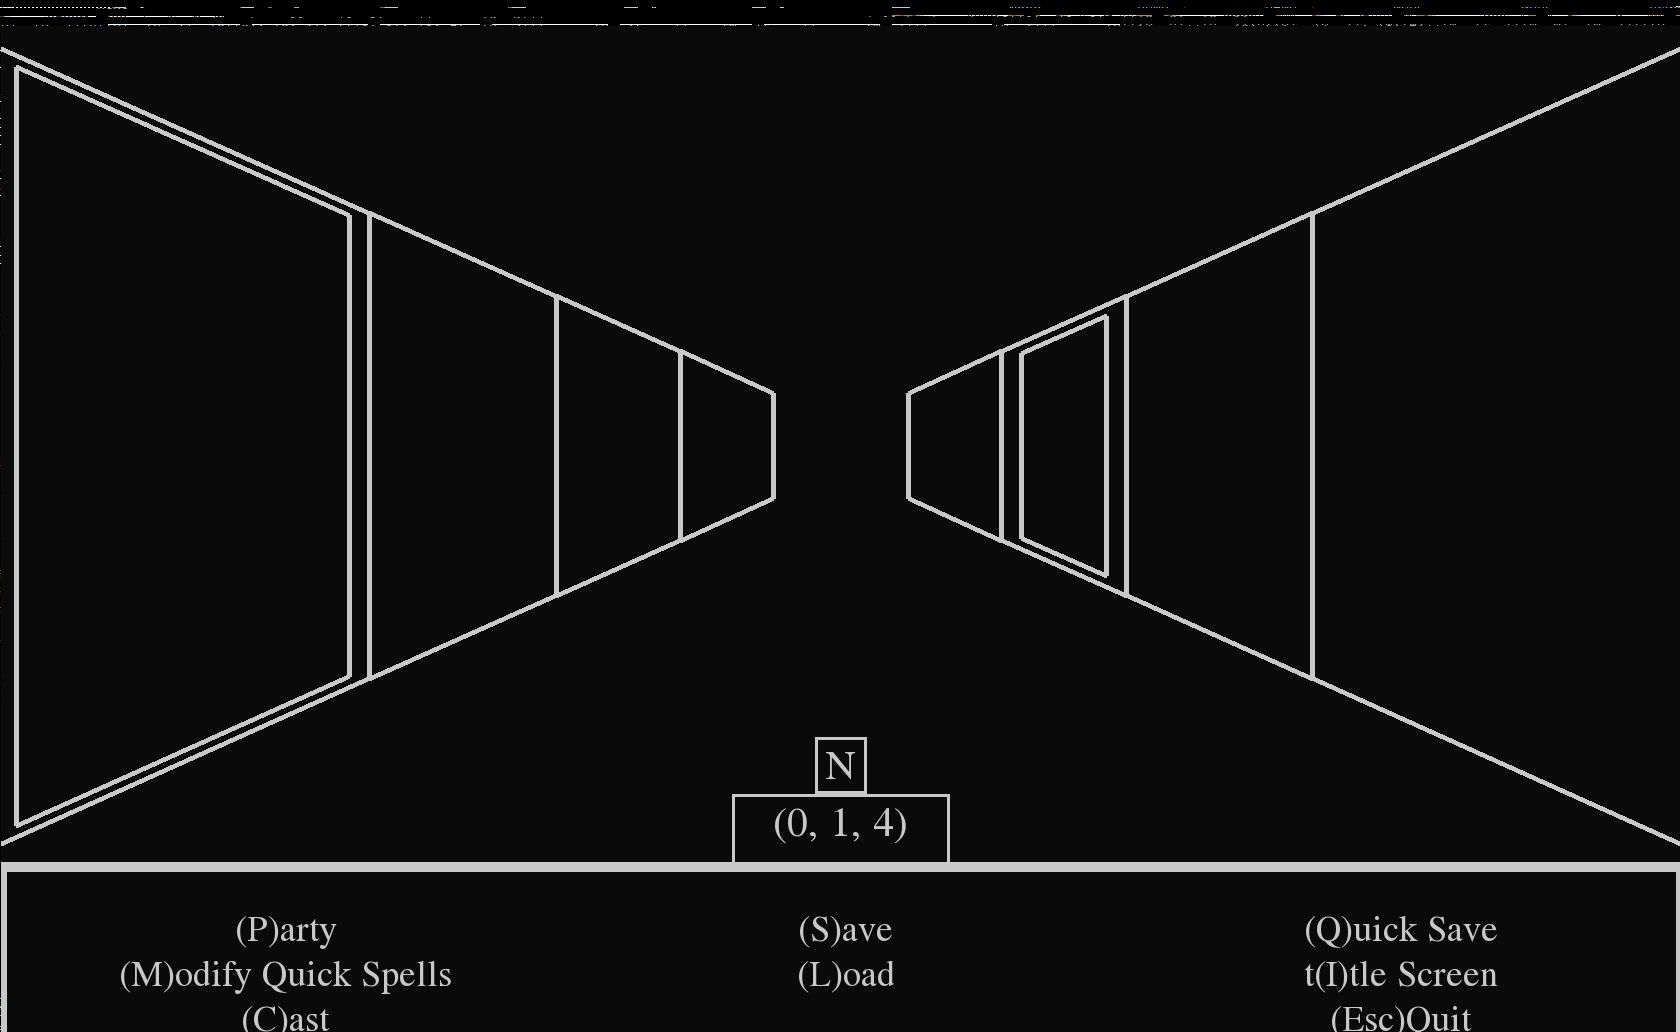
\includegraphics[width=\textwidth]{dungeon}
        \caption{Trebor Sux.}
        \label{fig_dungeon}
    \end{figure}

\section{Dungeon View}
In addition to the standard World View and Command View (see 
Chapter~\ref{ch_game_window}) there are two additional views:
\begin{itemize}
    \item Direction View - Indicates what direction you are facing: 
    North(\verb|N|), South(\verb|S|), East(\verb|E|), West(\verb|W|).
    \item Coordinate View - Tells you your current dungeon coordinates. Dungeons
    consist of a list of grids. Each grid corresponds to a floor of the dungeon. 
    Though each floor may vary in size, their maximum dimensions will be 
    $20\times 20$.
    Coordinate views are formatted as follows:
    $$(z,x,y)$$
    where $z$ is your current floor, $x$ is your current coordinate on the 
    horizontal axis, and $y$ is your current coordinate on the vertical axis. 
    All coordinates begin counting at $0$ (so a floor of dimensions
    $10\times 15$ will have $x$-coordinates from $0-9$ and $y$-coordinates from
    $0-14$). Meanwhile,
    if the dungeon has 5 floors, then the floors will range in number from
    $0-4$. Note that you may begin the dungeon on any one of the floors.

    In Figure~\ref{fig_dungeon}, the player is on floor 1, at horizontal-coordinate
    2, vertical-coordinate 4, and is facing North.
\end{itemize}

\section{Dungeon Commands}
    Observe in Figure~\ref{fig_dungeon} that there are no commands listed in the command view for moving. The player moves about using the arrow keys.
    \begin{itemize}
        \item {\color{green!50!black} $\uparrow$} - Move the party forward one step.
        \item {\color{green!50!black} $\downarrow$} - Move the party back one step.
        \item {\color{green!50!black} $\rightarrow$} - Turn the party to the right, but stay on the same square.
        \item {\color{green!50!black} $\leftarrow$} - Turn the player to the left, but stay on the same square.
        \item \verb|(P)arty| - See Chapter~\ref{sec_townmode}
        \item \verb|(S)ave| - See Chapter~\ref{sec_townmode}
        \item \verb|(L)oad| - See Chapter~\ref{sec_townmode}
        \item \verb|t(I)tle Screen| - See Chapter~\ref{sec_townmode}
        \item \verb|(C)ast| - Allows you to cast spells. Note that only buff
        (and perhaps some spectral spells) may be cast outside of combat. Outside
        of battle, a single round corresponds to a single \emph{movement} or
        \emph{change in direction}. In 
        other words, if you cast \verb|Shield| on yourself, and \verb|Shield| has
        duration 5, then you have five pushes of the arrow keys before 
        \verb|Shield| dissipates.
        \item \verb|(Esc) Quit| - See Chapter~\ref{sec_townmode}
    \end{itemize}

\section{Mapping}
    As can be seen from Figure~\ref{fig_dungeon}, the dungeon corridors look rather
    monotonous. Furthermore, many of the dungeons will be very confusing, with all
    sorts of twisting passageways, splits and dead-ends. Therefore, if you are going
    to have any hope of surviving the dungeons, you will need to create maps. 

    The best way to create maps is to get your hands on some graph paper, and
    use one sheet per floor. Then, when you first enter the dungeon, draw
    everything you can see. Each square on the walls corresponds to a single 
    square on your graph paper. Then, turn right/left, and write down what you
    see. Lather, rinse, and repeat until you've turned a full circle. Then, take a 
    step and do it again. Furthermore, make sure to periodically double-check
    that the coordinates on-screen correspond where you think you are on your map.

    It is also highly recommended that you mark on your map important places,
    such as the exit from the dungeon (if any) any healing or rest spots, important
    events, etc.

\section{Fancy X's}
Frequently, while wandering through the dungeons you'll stumble upon strange \emph{X}'s marked on the floor (see Figure~\ref{fig_x}. When you step on the \emph{X} something will happen. What happens
depends on the color of the \emph{X}:

\begin{itemize}
    \item \textcolor{red}{Red} - When you step on this square, violence will ensue.
    \item Grey - Stepping on this square will unlock a new command \verb|(D)own|, that allows you to descend to the floor below the current one. If you see this \emph{X} on the ceiling, 
        then stepping
        beneath it will unlock the command \verb|(U)p|, and allow you to ascend to the floor above the current one.
    \item \textcolor{blue}{Blue} - An event of some kind. Usually some sort of scene with dialog. May lead to combat.
    \item \textcolor{green}{Green} - Used to represent an exit from the dungeon. Stepping on this square will unlock the command \verb|(E)xit|, which allows you to leave the dungeon, and return to
        town.
\end{itemize}

\begin{figure}[h!]
    \includegraphics[width=\textwidth]{herebedragons}
    \caption{Here be dragons.}
    \label{fig_x}
\end{figure}
    

\chapter{Combat}
\label{ch_combat}
\epigraph{Watch your enemies carefully. See how they fight. See how
they interact with their allies. This will give you hints to their strengths and
weaknesses. Once you've found a weakness, exploit it mercilessly!}{Reyna of 
Chengue} 

Ah, combat. The part that puts ``game" in ``computer role-playing game." Combat
is broken into rounds. At the beginning of each round, the player selects the 
actions for each member of her party, while the computer selects options for the
player's opponents (how smart the computer is depends on the difficulty. On easy
difficulties, the computer's a moron, on higher difficulties, the computer is
slightly smarter).

\section{Armslength vs. Grappling}

There are two combat styles:
\begin{itemize}
    \item Armslength
    \item Grappling
\end{itemize}

Each combat style caters to different strengths. Armslength is the default combat
style. It's where enemies have some small distance between them. Basically, combatants are too far
away to bite each other. When two opponents grapple, however, they are getting
up close and personal (biting range).

Armslength is a good place to be for characters who wield spears, or cast 
multi-target spells. Spears receive bonuses to attack and damage when wielded at
armslength, but receive penalties to the same when the wielder is grappling. 
Meanwhile, most multi-target spells may only target multiple targets when the 
caster is at armslength. As soon as the caster is grappled, she may only target
her grappled opponent (or herself, if the spell is beneficial).

Grappling, meanwhile is very useful for characters who use daggers, and have a 
high magic, but aren't the party's artillery. Daggers receive bonuses to attack
and damage while the wielder is grappling, and penalties while she is at
armslength. Meanwhile, a grappler with high magic can very effectively shut down
a dangerous spellcaster, while her allies deal with the spellcaster's companions.

Swords are grapple agnostic. They are equally effective both at armslength and
while grappling. As such, swordsmen (and women) are very versatile, though they rarely have the 
same level of damage output as their spear and dagger wielding counterparts.

\section{Combat Options}

Figure~\ref{fig_combat} displays a potential combat screen.


\begin{figure}[h!]
    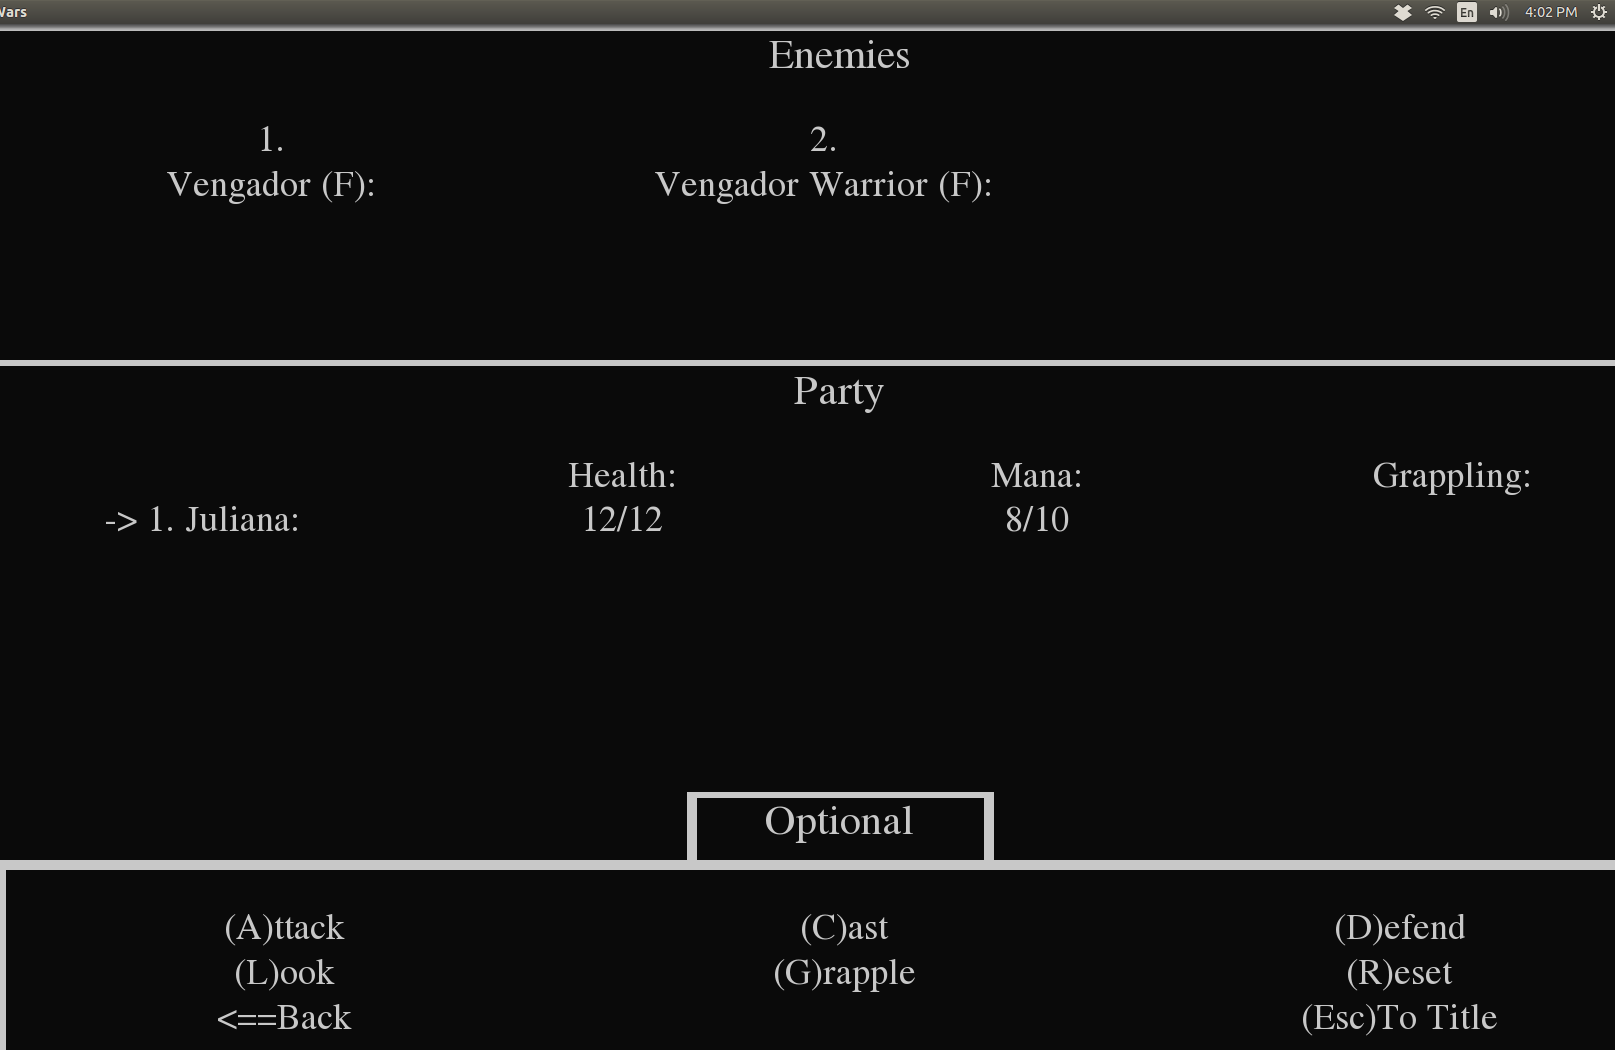
\includegraphics[width=\textwidth]{combat}
    \caption{A Slime draws near! Command?}
    \label{fig_combat}
\end{figure}

Observe the arrow {\color{green!50!black} \texttt{->}} pointing towards Juliana's name. The arrow tells you which character is currently being given commands. 
The \verb|Grappling| column tells you which enemy each party member is grappling, if any\footnote{Currently, enemies of the same type are not distinguished between each
other. This
can make it difficult to tell precisely which enemy is being grappled when fighting two of the same type. This will be rectified at some point in future updates}.

The following commands are available while fighting at arms length:
\begin{itemize}
    \item \verb|(#Enter) Attack| - Attack an enemy with your equipped weapon. If you press \verb|Enter| the game automatically targets the first enemy. If you press a number, then your character
        will target the enemy with the associated number.
    \item \verb|(C)ast| - Cast a spell. When targeting multi-target spells, an \verb|X| will appear next to enemies that have
    already been targeted.
    \item \verb|(D)efend| - Defend. Note that defending increases your character's
    warfare, grapple, and magic by 3. Very useful when your character has been
    inflicted by a negative status!
    \item \verb|(L)ook| - Allows you to look at your opponents. Note that you can
    look at your enemies \emph{for free.} Looking \emph{does not} count as a round
    of combat. Looking can be very valuable when determining what your enemies are
    good at. If your enemy is wielding a spear, chances are they're not so good
    at grappling.
    \item \verb|(G)rapple| - Try to initiate a grapple with an opponent.
    \item \verb|(B)reak Ally's Grapple| - Only available if one of your allies is grappled.
    This allows you to attempt to break that grapple, and force your ally's grappler
    to grapple you instead. Very valuable if your artillery has been 
    grappled by your enemy's grapple tank!
    \item \verb|(S)pank| - Only available when grappling. Allows you to give your opponent a quick spanking. If successful, your opponent will become humiliated and lose focus, giving them a -1 
        penalty to all primary stats. However, there is a chance that your opponent will reverse the spanking, so be careful.
    \item \verb|(F#) Quick Spell| - When you press one of the function keys (F1, F2, etc.), the player will cast the associated quick spell (though you will still have to select a target(s) for the spell).
    \item \verb|(R)eset| - Clears all of your character's options, and allows you
    to start again. Note that this \emph{does not} restart combat. It only 
    clears your choices for the current round.
    \item {\color{green!50!black} \texttt{<==}} - Go back to the previous 
        character.
    \item \verb|(Esc) To Title| - Exit combat and return to title screen.
    \item \verb|(R)un| - Not displayed in Figure~\ref{fig_combat}. Allows you
        to try run away from combat like the cowardly dog you are.
\end{itemize}

The following commands are available while grappling:
\begin{itemize}
    \item \verb|(A)ttack| - See above.
    \item \verb|(C)ast| - See above. Note that most of the time you will only
    be able to target either your enemy, or yourself while grappling.
    \item \verb|(D)efend| - See above.
    \item \verb|(L)ook| - See above.
    \item \verb|Throw| - Allows you to throw your grappled opponent at another
    opponent, doing damage to both! (Note: Your grappled opponent may also be "thrown" at
    themselves. This is basically telling your character to throw them against
    a wall or something). Note that this command breaks the grapple, but is harder
    to pull off than the \verb|(B)reak Grapple| command.
    \item \verb|(B)reak Grapple| - Attempt to end the grapple.
    \item \verb|(R)eset| -  See above.
    \item {\color{green!50!black} \texttt{<==}} - See above.
    \item \verb|(Esc) To Title| - See above.
\end{itemize}

\section{Victory and Character Improvements}
Yay! You have emerged victorious! The victory jingle plays, you rub your hands
together, and you look forward to some sweet, sweet exp-

Hey, where's the experience?

Well, unlike most RPG's, this game doesn't work off of experience. Rather, your
characters' stats have a chance of increasing depending on what you do in 
combat (very similar to \textit{Final Fantasy Legend II} for the Gameboy).

\subsection{Stat Improvements}
The stats increase as follows:
\begin{itemize}
    \item \verb|Strength| - Increases if you attack often
    \item \verb|Willpower| - Increases if you cast status spells (explained below) often, or if you defend.
    \item \verb|Dexterity| - Increases if you use grappling actions 
    (grapple, break grapple, throw), or if you attack while grappled.
    \item \verb|Alertness| - Flat chance of increasing every combat\footnote{
Starting with the second episode, there will be a new command "Hide" that allows you to ambush your opponents (or just not get attacked). Hiding will increase stealth.}
    \item \verb|Talent| - Increases if you cast spells
    \item \verb|Health| - Flat chance of increasing every combat. Has a higher
    chance of increasing if the player attacks/grapples often.
    \item \verb|Mana| - Flat chance of increasing every combat. Has a higher
    chance of increasing if the player casts spells often.
\end{itemize}


\subsection{Learning Spells}

This is about learning spells. For more details about spells, see Chapter~\ref{ch_spells}.

Spells are broken into four schools: Combat, Status, Buff, and Spectral. For 
details about each school, see Chapter~\ref{ch_spells}


You learn spells of a given type by casting the spell of that type. So in order to learn Icebolt, you need to be casting Firebolt.  Casting Firebolt will not allow you to learn Mass Weaken. Only casting Weaken will get you Mass Weaken.

\subsubsection{Tiers}
Spells are further broken into tiers: 0 - 9.

Each tier has three spells: Basic, Advanced, Specialized. As per the name, specialized is available only if your character specializes in that school (the path to specialization will begin in the second episode). You must learn the basic spell before you learn the advanced spell, and the advanced spell before you learn the specialized spell. Advanced and specialized spells tend to be stronger and/or cheaper versions of the basic spell. Firebolt is the basic tier 0 combat spell, Icebolt is the advanced tier 0 combat spell. Magic bolt is the specialized tier 0 combat spell (at this point, you've only seen Magicbolt used against you).


Every 3 levels of magic\footnote{This will change. Based upon how stats are increasing in the first episode, if I keep this across the board, you'll be learning Tier 9 spells by about a third of the way through the game. At that point, you should be only up to Tiers 3-4.} 
a new tier opens up. Note that you do not need to learn all the spells of a lower tier to begin learning spells of a higher tier. You learn spells of a higher tier the same way you learn advanced spells of a lower tier: cast spells of the appropriate type. So if you want to learn Distort Magic (which is a Status spell) you first need to get your magic up to three, and then cast Weaken/Mass Weaken a bunch of times.  
When learning spells, it does not matter which spell of the appropriate school that you cast. Once you've unlocked Tier 9, you will be able to learn Tier 9 combat spells by just slinging Firebolts all over the place. On the other hand, if you haven't learned Icebolt, and you start slinging Tier 8 spells around, you may learn Icebolt rather than a Tier 9 spell. However, you have a better chance of learning higher tier spells than learning lower tier spells (assuming the higher tier spells are available to you). So if you unlock Tier 1, and you haven't learned Icebolt yet, you'll have a better chance of learning Lightning Bolt than of learning Icebolt.

\section{Defeat and Second Chances}

You've lost! Oh, woe is you! How will you look your family in the eye? 
Fortunately, if you are defeated, you'll get sad music playing, and then you'll
be given the option to try the fight again. If you choose to try again, the fight
resets the state you were in at the beginning of the fight, and you can either
try to defeat your enemies, or run away if that option is available.

If you choose not to try again, then you will return to the Title Screen, from
which you can load your last save game, or close the game in frustration and 
unleash a stream of curse words at me. Such is the sacrifice I make for the craft.

However, if you look at Figure~\ref{fig_combat}, you will see the word 
\verb|Optional| wrapped in a box. If you see this during the round, it means that
the fight does not need to be won to complete the game. For fights with the
\verb|Optional| tag, if you choose not to try again, you will get a different
post-combat scene than if you won, and then the game will continue like normal.
Typically, boss fights will
be optional, because those fights will be geared more towards the truly dedicated
RPGers, as opposed to the more casual
gamers who are just in it for the spankings (not to say the hard-core players 
aren't in it for the spankings too. You can enjoy both after all).

\chapter{Spells}
\label{ch_spells}
\epigraph{\emph{Never} underestimate the devastating power of the right spell at the right time. You know how you hear about those super-experienced adventurers who triumph
over impossible odds? Nine times out of ten, they won because they knew which spell to cast when.}{Reyna of Chengue}

Ah, magic. The best part about fantasy-based CRPG's. Grappling, and armslength is nice, but it is here with magic that the true depth of gameplay makes itself 
known. Which spell to cast? How often should you cast it? Should you try to conserve mana? Should you cast the cheap, but weak spell, or the strong but powerful spell?
Is there a cheap spell that is actually \emph{more} effective against this enemy than the expensive but powerful spell? Is this battle so damned hard because it's just
that hard, or because I'm not casting the right spells? Such are but a small sampling of the types of questions that run through a player's mind when playing a well-made
RPG (so, if these questions aren't running through your mind, please let me know). 

\section{Spell Schools}
\label{sec_schools}
Spells are broken into four schools, based on what they accomplish.
\begin{itemize}
    \item \verb|Combat| - Deal straight damage. Tend to be expensive, but can be devastating, especially against enemies with low magic. \verb|Firebolt| is the first 
    combat spell.
    \item \verb|Status| - Interfere with your opponent's ability to fight (reducing stats, paralyzing them, etc.). \verb|Weaken| is the first status spell.
    \item \verb|Buff| - Improves your characters' abilities to fight (also includes healing spells). \verb|Heal| is the first buff spell.
    \item \verb|Spectral| - Weird spells. Typically have more than one effect (i.e. damage plus a status effect), or allow spellcasters to "simulate" other combat actions using a different stat rather than the stat the other action depends on. \verb|Spectral Spanking| is the first spectral spell (Spectral Spanking simulates the \verb|Spank| 
    option, but uses \verb|magic| rather than \verb|grapple| to determine the chances of success. Furthermore, your opponent cannot reverse a Spectral Spanking).
\end{itemize}

\section{Spell Information}

The player is capable of looking at the stats of her spells in game. Therefore, the specific details of each spell will not be reproduced here. However, we will explain
how to read the notation used to keep the spell descriptions concise. Consider Figure~\ref{fig_spell}.

\begin{figure}[h!]
    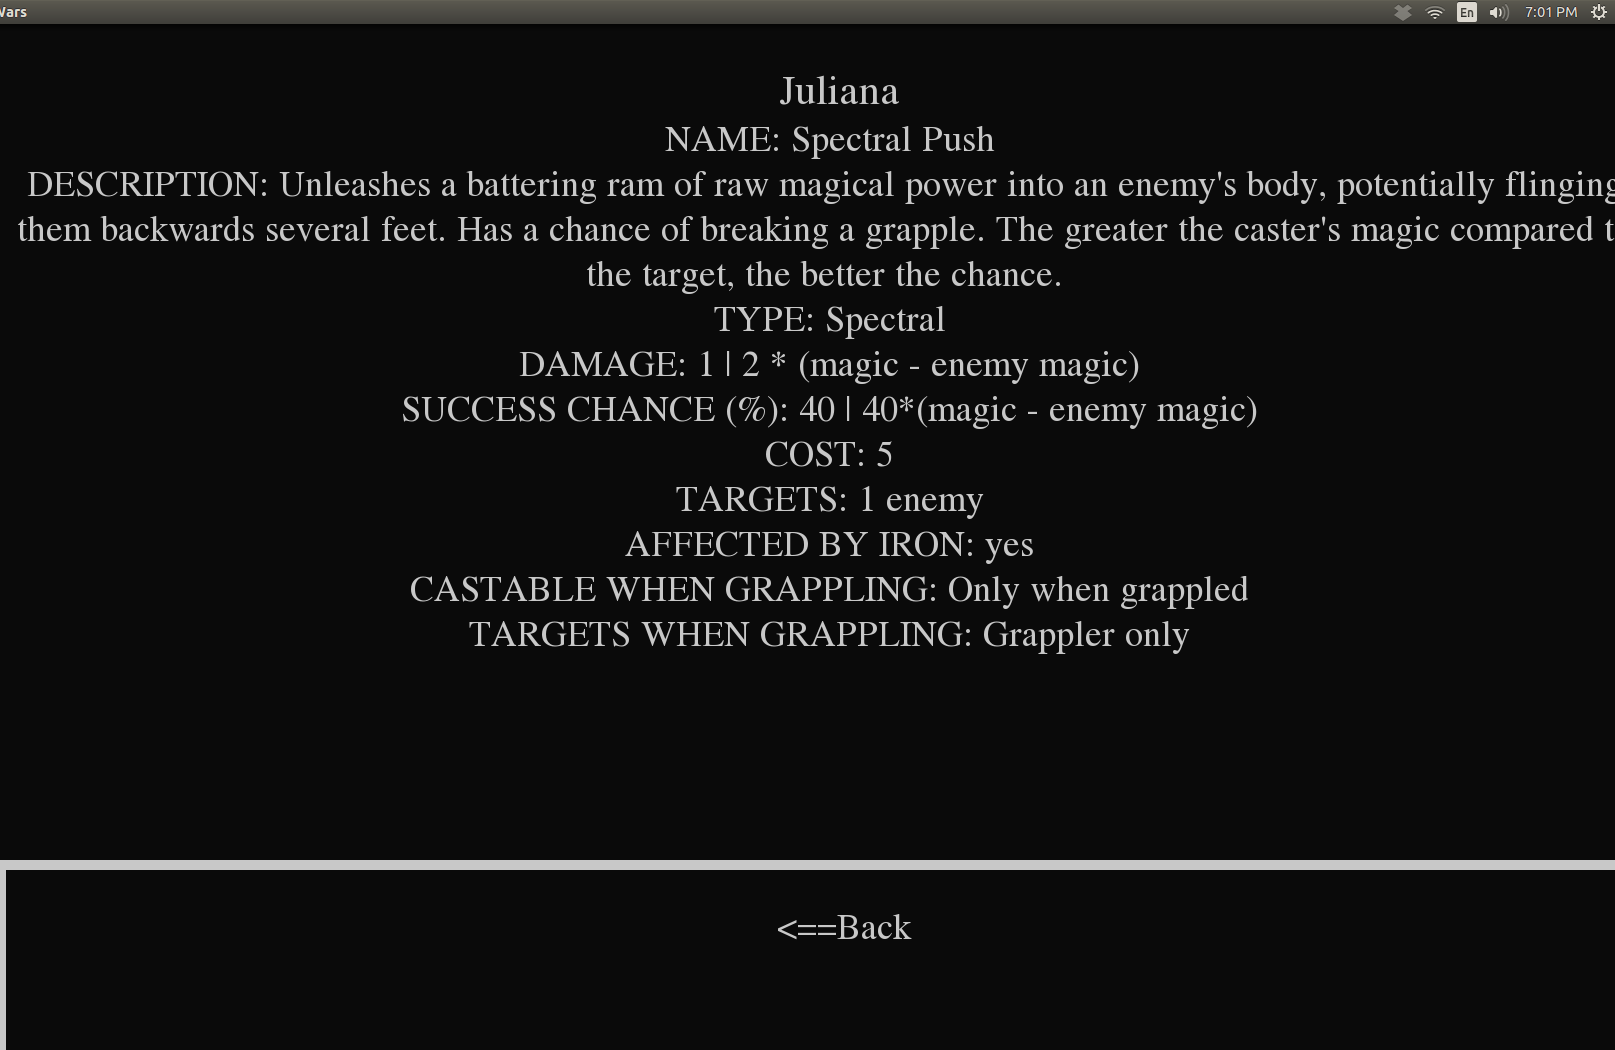
\includegraphics[width=\textwidth]{spell}
    \caption{Good for curing constipation too.}
    \label{fig_spell}
\end{figure}


\begin{itemize}
    \item \verb|NAME| - The name of the spell.
    \item \verb|DESCRIPTION| - A brief description of the spell in English.
    \item \verb|TYPE| - The spell school (see Section~\ref{sec_schools}).
    \item \verb|DAMAGE| - How much damage the spell can do. The damage is specified
    as a range. $1 \mid 2*(\mathit{magic} - \mathit{enemy~magic})$ indicates that the
    spell's damage ranges from to two times the difference between your magic
    and your enemy's magic. If $1 > 2*(\mathit{magic} - \mathit{enemy~magic}$, then
    the spell does $1$ damage. You may also see ranges of the form
    $x \mid y \mid z$. This means that the spell will do at least $x$ damage, at most
    $z$ damage, and $y$ damage otherwise. 
    %\item \verb|SUCCESS CHANCE(%)| - How likely the spell is to succeed at 
    %inflicting at some action outside of damage (in the case of Spectral Push, of 
    %breaking a grapple).
    \item \verb|COST| - How much mana the spell costs.
    \item \verb|TARGETS| - The maximum number of targets the spell has, and whether the spell
    targets allies or enemies.
    \item \verb|AFFECTED BY IRON| - Iron interferes with magical currents. 
    As a result, any spell that strikes a character with raw magical power (such
    as all spectral spells) will suffer penalties if cast on a character wearing
    iron armor. This \emph{includes} beneficial spells like \verb|Heal|. The only
    exception to this is if a caster is targeting themselves. Then, since the 
    spell energy never actually leaves the caster's body, the iron doesn't 
    interfere, and the spell works at full power.

    So suppose Pat the Paladin is clad in full plate mail. Then, if Heather the 
    Healer casts \verb|Heal| on Pat, Heather's heal spell will be weakened, and she will
    heal much less than would be expected based on her magic stat. If on the
    other hand, Pat casts \verb|Heal| on himself, then he will heal himself at full
    power.

    Meanwhile, if Bob the Battlemage casts \verb|Firebolt| on Peter, the spell will still
    do full damage, because magic is only used to start (and maintain) the fire.
    Pat will still be hurt because the flames will heat his armor, and burn his
    precious flesh (which will then be perfectly healed by his health,
    allowing us to have a bunch of beautiful people burning and hacking at each
    other without any of them becoming horribly scarred).

    \item \verb|CASTABLE WHEN GRAPPLING| - Determines how this spell interacts with
    grappling. The possible grappling statuses are: \verb|Only when grappled|, 
    \verb|Not when grappled|, \verb|Yes|. 
        \begin{itemize}
            \item \verb|Only when grappled| - This spell may only be cast when
            the caster is grappled.
            \item \verb|Not when grappled| - This spell can't be cast at all
            when grappled
            \item \verb|Yes| - This spell may be cast while grappling.
        \end{itemize}
    \item \verb|TARGETS WHEN GRAPPLING| - Determines how the spell's targeting
    interacts with grappling. The options are: \verb|Grappler only|, \verb|Anyone|,
    \verb|No|
    \begin{itemize}
        \item \verb|Grappler only| - Spell may only target self or grappler.
        \item \verb|Anyone| - Spell's targeting unaffected by grappling.
        \item \verb|No| - Spell cannot target anyone while caster is grappling.
    \end{itemize}
\end{itemize}

\section{Quick Spells}

To make combat more streamlined, the game allows you to save up to 12 spells as quick spells, which may be accessed by the function keys (F1 - F12). You may modify the quick spells at any time 
outside of combat with the \verb|(M)odify Quick Spells| command. The Modify Quick Spells menu will show each of the twelve function keys, along with the spell it is assigned to (or \verb|None|) if
the slot is empty. You can swap two spells by selecting the first, and then the second. Or you can assign a spell to a given slot by pressing the appropriate function key, and then selecting a spell
just like you would in combat.

Note that each time you learn a spell, the spell is automatically added to the first empty function key, so long as there is at least one empty function key.

\chapter{Acknowledgements}

It's impossible to accomplish a project of this scale without help, and I'd like to offer thanks to those who have helped me (directly and indirectly) in developing this game.


Starting with Episode 2, Emily of AnimeOTK will be serving as editor. Thank you Emily!

Uninventive, Johny741, and a mysterious man I've named Jeffrey the Jungle-Ape have agreed to be my beta testers. Thanks to all of you for your patient bug finding!

The game is written using the game engine \href{www.pygame.org}{Pygame} in \href{www.python.org}{Python 2.7}. This manual was typset using \LaTeX. The fancy colors and 
layout are thanks to the \href{texcatalogue.ctan.org/entries/pdfscreen.html}{pdfscreen} package.

All in-game music was purchased from \url{www.playonloop.com}.

Finally, thank you, the reader, for taking the time to play \textit{Pandemonium Cycle: The Potion Wars}. I hope you enjoy it! 

\end{document}
